\subsubsection{Structure from motion}
Jedną z funkcjonalności oferowanych przez przygotowane oprogramowanie jest wyznaczanie struktury przestrzennej sceny w postaci chmury punktów na podstawie zbioru fotogramów przy pomocy techniki Structure from motion. Zaproponowana implementacja opiera się na wykorzystaniu popularnego narzędzia COLMAP\cite{schoenberger2016mvs}\cite{Schonberger_2016_CVPR}, które zostało włączone do projektu w postaci pythonowej biblioteki \href{https://github.com/colmap/pycolmap}{\textit{pycolmap}}. Biblioteka ta oferuje szereg funkcji umożliwiających przeprowadzenie kluczowych etapów procesu SfM, w tym wykorzystane w projekcie funkcjonalności do wykrywania cech charakterystycznych na obrazach, dopasowywania punktów wspólnych między obrazami czy przeprowadzania inkrementalnej rekonstrukcji, która dodatkowo została skonfigurowana za pomocą parametrów dobranych tak, aby zapewnić zadowalającą jakość wyniku przy zachowaniu wydajności.

W wyniku działania tak zaimplementowanego procesu powstają pliki binarne zapisujące dane przede wszystkim wyznaczonych punktów 3D i pozycji kamer. Biblioteka \textit{pycolmap} umożliwiła dodatkowo łatwe wprowadzenie funkcjonalności eksportu wyników do formatu PLY, którego to formatu plik zostaje wykorzystany do wizualizacji wygenerowanej chmury punktów. Z kolei reprezentacja w postaci plików binarnych zostaje w kolejnych etapach wczytywana i po przefiltrowaniu służy za podstawę do modelowania z zastosowaniem algorytmu Gaussian Splatting.

\begin{figure}[!ht]
  \centering
  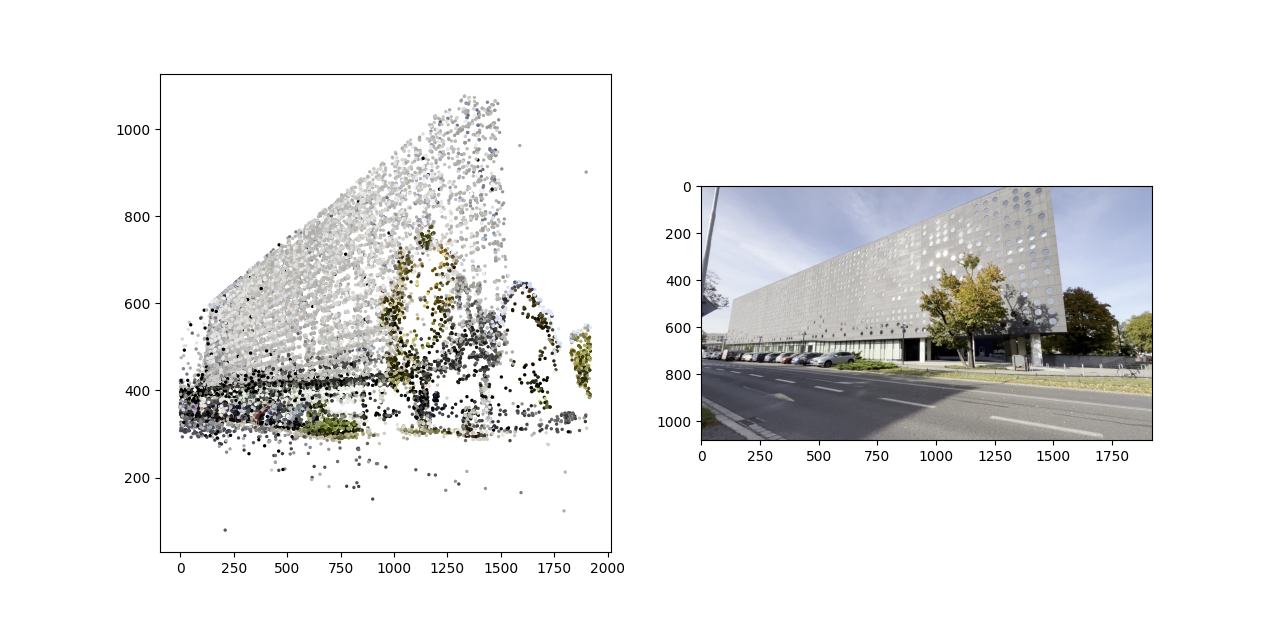
\includegraphics[width=0.9\linewidth]{img/sfm_projection.png}
  \caption{Projekcja przykładowej chmury punktów na płaszczyznę porównana do zdjęcia}
\end{figure}